\section{SAT model}

The resolution of the problem is approached following two models.

\begin{itemize}
    \item \textbf{Unified model}:
    based on the definition of two decision variables \texttt{assignments} and \texttt{paths}.
    \item \textbf{Matrix model}:
    based on the definition of one decision variable $X$.
\end{itemize}

Some modifications were applied to those model in order to visualize eventual differences in terms of performances.

The discussion is going to be much more focused on the Unified model just to mantain a logical thread within the explication of models used for other solvers.

\subsection{Unified Model}

\paragraph*{General Definition}
The Unified model aims to find the correct assignment to both decision variables, in such a way that it satisfy all constraints.\\
The idea behind this kind of model is based on the separation of the two task just specified in one.

\paragraph*{Original Workflow}
The original workflow follows the next steps:
\begin{enumerate}
    \item find satisfying values for the \texttt{assignments} variable, else end the algorithm
    \item find satisfying values for the \texttt{paths} variable, else proceed to step $4$
    \item repeat step $2$ to find a new optimized solution,
    \item repeat step $1$ just to find another assignment
\end{enumerate}

\paragraph*{New Workflow}
The new algorithm simply tries to optimize the assignment to both variable.

\paragraph*{Pro}
The model was designed to improve certain intrinsic problems of the definition of a problem through SAT:
\begin{itemize}
    \item \textbf{Specificity of constraints}: constraining much more the assignments of the two variable guarantes to mantain lower width of exploration of the resolution tree.
\end{itemize} 

\paragraph*{Contro}
The model falls into a few issues such:

\begin{itemize}
    \item \textbf{Dimension}: being based on two decision variables, the dimension of the problem scale exponentially with them. \footnote{The scaling dimension of the problem implies higher needs of time to build the model.}
\end{itemize}

\subsubsection{Decision variables}

\begin{itemize}
    \item \texttt{assignments}: $n \times m$ boolean matrix
    \begin{equation}
        \label{eq:assignments}
        \texttt{assignments[$p$, $c$] = 1 }
        % \quad
        % \texttt{if courier $c$ delivers pack $p$}
    \end{equation}
    \begin{center}
        \texttt{if courier $c$ delivers pack $p$}
    \end{center}

    \item \texttt{paths}: $m \times (n+1) \times (n+1)$ boolean matrix
    \begin{equation}
        \label{eq:paths}
        \texttt{paths[$c$, $loc_1$, $loc_2$] = 1 }
    \end{equation}
    \begin{center}
        \texttt{if courier $c$ moves from location $loc_1$ to $loc_2$}
    \end{center}

    \item \texttt{u}: $m \times n \times n$ boolean matrix\footnote{The definition of the \texttt{u} variable is useful for the MTZ formulation.}
    \begin{equation}
        \label{eq:u}
        \texttt{u[$c$, $p_1$, $p_2$] = 1 }
    \end{equation}
    \begin{center}
        \texttt{if in the courier $c$ path the node $p_1$ is associated to value $p_2$}
    \end{center}
    
\end{itemize}

\subsubsection{Objective function}

The model aims to minimize the maximum distance travelled by any courier.
The objective function can estimated as the maximum between the total distances of each courier:

\begin{equation}
    \label{eq:obj_fun}
    \max_{c \in \{ 1, \dots, m \}}
    \sum_{loc_1=1}^{n+1} \sum_{loc_2=1}^{n+1} \texttt{D[$loc_1$, $loc_2$]}*
    \texttt{paths[$c$, $loc_1$, $loc_2$]}
\end{equation}

A lower bound is set to costrain the objective during the resolution phase.
\begin{equation}
    \label{eq:lower_bound}
    \max_{p \in \{ 1, \dots, n \}}
    \texttt{D[$n+1$, $p$] + D[$p$, $n+1$]}
\end{equation}
Its value is hypotesized to be the maximum between the minimum distance paths that a courier can travel. And this can be computed as the distance needed for a courier to reach a certain pack and return to the depot.



\subsubsection{Constraints}

\paragraph*{Assignment related constraints}

\begin{itemize}
    \item Capacity constraint:
    \begin{itemize}
        \item Sum of sizes of packs delivered by a singular courier must be under its load limit
        \begin{equation}
            \label{eq:capacity1}
            \forall c \in \{1 \ldots m\}:
            \quad
            \sum_{p=1}^{n} \texttt{assignments[$p$, $c$] * sizes[$p$]} \leq \texttt{loads[$c$]}
        \end{equation}
        \item Each pack must be delivered only by a courier
        \begin{equation}
            \label{eq:capacity2}
            \forall p \in \{1, \ldots, n\}: \exists! c \in \{1, \ldots, m\} \quad \texttt{s.t.} \quad \texttt{assignments[$p$, $c$]} = \texttt{1}
        \end{equation}
    \end{itemize}
\end{itemize}

\paragraph*{Path related constraints}

\begin{itemize}
    \item General path constraints
    \begin{itemize}
        \item If courier delivers at least one package, there must exist a destination from DEPOT\footnote{DEPOT is the original position, hypotesized as \texttt{n+1}.} with true value, else it can stay in DEPOT
        \begin{equation}
            \label{eq:gen_path_constr1}
            \forall c \in \{1 \ldots m\}:
            \forall p \in \{1 \ldots n\}:
            \left\{
                \begin{array}{lr}
                    \texttt{NOT(paths[$c$, DEPOT, DEPOT])} & \texttt{iff } \sum_{p=1}^{n} \texttt{assignments[$p$, $c$]} \geq \texttt{1}\\
                    \texttt{paths[$c$, DEPOT, DEPOT]} & \texttt{iff } \sum_{p=1}^{n} \texttt{assignments[$p$, $c$]} = \texttt{0} % or otherwise
                \end{array}
            \right\}
        \end{equation}

        \item If courier delivers pack p, its destination must be different from p 
        \begin{equation}
            \label{eq:gen_path_constr2}
            \forall c \in \{1 \ldots m\}:
            \forall p \in \{1 \ldots n\}:
            \left\{
                \begin{array}{lr}
                    \texttt{NOT(paths[$c$, $p$, $p$])} & \texttt{iff } \texttt{assignments[$p$, $c$]}\\
                    \texttt{paths[$c$, $p$, $p$]} & \texttt{iff } \texttt{NOT(assignments[$p$, $c$])} % or otherwise
                \end{array}
            \right\}
        \end{equation}

        \item Each pack must be delivered by a single courier only once
        \begin{equation}
            \label{eq:gen_path_constr3}
            \forall c \in \{1 \ldots m\}:
            \forall loc_1 \in \{1 \ldots n+1\}:
            \quad
            \sum_{loc_2=1}^{n+1} \texttt{paths[$c$, $loc_1$, $loc_2$]} = \texttt{1}
        \end{equation}
    \end{itemize}
    \item Subcircuit constraints
    \begin{itemize}
        \item Only a single courier must deliver pack in location $loc_2$ from $loc_1$
        \begin{equation}
            \label{eq:subtour_constr1}
            \forall c \in \{1 \ldots m\}:
            \forall loc_2 \in \{1 \ldots n+1\}:
            \quad
            \sum_{loc_1=1}^{n+1} \texttt{paths[$c$, $loc_1$, $loc_2$]} = \texttt{1}
        \end{equation}
        \item Subtour elimination
        \begin{itemize}
            \item $u$ relative to first pack $p$ of courier $c$ path must have value = 1
            \begin{equation}
                \label{eq:subtour_constr2}
                \forall c \in \{1 \ldots m\}:
                \forall p \in \{1 \ldots n\}:
                \quad
                \texttt{iff}
                \quad
                \texttt{paths[$c$, DEPOT, $p$]}
                \quad
                \texttt{then}
                \quad
                \texttt{u[$c$, $p$, $1$]}
            \end{equation}
            \item $u_j \geq u_i + 1$
            \begin{equation}
                \label{eq:subtour_constr3}
                \forall c \in \{1, \dots, m\}: \ \forall i, j, k \in \{1, \dots, n\}: \quad
                \texttt{paths}[c, i, j] \land \texttt{u}[c, i, k] \Longrightarrow
                \sum_{l=k+1}^{n} \texttt{u}[c, j, l] = 1
            \end{equation}
            
            \item Exatcly one true value for each \texttt{u[$c, p, :$]} vector
            \begin{equation}
                \label{eq:subtour_constr4}
                \forall c \in 1 \ldots m:
                \forall p_1 \in 1 \ldots n:
                \quad
                \sum_{p_2=1}^{n} \texttt{u[$c$, $p_1$, $p_2$]} = \texttt{1}
            \end{equation}

            \item MTZ formulation constraint:
            \begin{center}
                $u_i - u_j + 1 \leq (n - 1)$ * $(1 - paths[c, i, j] )$
            \end{center}
            \begin{equation}
                \label{eq:subtour_constr5}
                \forall c \in \{1, \dots, m\}, \ \forall i, j, k_1, k_2 \in \{1, \dots, n\}: 
            \end{equation}
            \begin{center}\[
                \quad
                \texttt{u}[c, i, k_1] \land \texttt{u}[c, j, k_2] \Longrightarrow
                (k_1 - k_2 + 1) \leq (n-1) \cdot (1 - \texttt{paths}[c, i, j])
                \]
            \end{center}
        \end{itemize}
    \end{itemize}
\end{itemize}

\paragraph*{Symmetry breaking constraint}

A possible way to reduce tree exploration is to introduce symmetry breaking constraints.
One of them in this case can consist in constraining the order of assignments of packs between couriers with the same amount of load capacity.

But the experimentation didn't lead to major improvements.

\subsection{Validation}

\subsubsection*{Experimental design}

Some modifications were applied to the basic model in order to visualize eventuale differences in performances.
The original Unified Model was modified in three different versions:
\begin{itemize}
    \item Unified Model with Symmetry Breaking Constraint
    \item Unified Model with Cumulative Constraint Application
    \item Unified Model with Heule Encoding approach for \texttt{at\_most\_one()}
\end{itemize}
\subsubsection*{Experimental results}

As we can notice from the following table the performances were not very much different from the basic model. Only in the first 10 instances it has been possible to rach at least a suboptimal solution, while for the remaining ones the construction of the model required too much time causing the exceeding of the timeout limit.
\begin{table}[h]
    \centering
    \begin{tabular}{cccccc}
            \toprule
            Id & un-model & un-symm-model & un-cum-constr-model & un-heule-enc-model & matrix-model \\ 
            \midrule
            1 & \textbf{14} &       \textbf{14} &   \textbf{14} &   \textbf{14} &   \textbf{14} \\ 
            2 & \textbf{226} &      \textbf{226} &  \textbf{226} &  \textbf{226} &  \textbf{226} \\ 
            3 & \textbf{12} &       \textbf{12} &   \textbf{12} &   \textbf{12} &   \textbf{12} \\ 
            4 & \textbf{220} &      \textbf{220} &  \textbf{220} &  \textbf{220} &  \textbf{220} \\ 
            5 & \textbf{206} &      \textbf{206} &  \textbf{206} &  \textbf{206} &  \textbf{206} \\ 
            6 & \textbf{322} &      \textbf{322} &  \textbf{322} &  \textbf{322} &  \textbf{322} \\ 
            7 & 232 &       238 &   222 &   296 &   292 \\ 
            8 & \textbf{186} &      \textbf{186} &  \textbf{186} &  \textbf{186} &  \textbf{186} \\ 
            9 & \textbf{436} &      \textbf{436} &  \textbf{436} &  \textbf{436} &  \textbf{436} \\ 
            10 & \textbf{244} &     \textbf{244} &  \textbf{244} &  \textbf{244} &  \textbf{244} \\ 
            11 & -- &       -- &    -- &    -- &    -- \\ 
            12 & -- &       -- &    -- &    -- &    -- \\ 
            13 & -- &       -- &    -- &    -- &    -- \\ 
            14 & -- &       -- &    -- &    -- &    -- \\ 
            15 & -- &       -- &    -- &    -- &    -- \\ 
            16 & -- &       -- &    -- &    -- &    -- \\ 
            17 & -- &       -- &    -- &    -- &    -- \\ 
            18 & -- &       -- &    -- &    -- &    -- \\ 
            19 & -- &       -- &    -- &    -- &    -- \\ 
            20 & -- &       -- &    -- &    -- &    -- \\ 
            21 & -- &       -- &    -- &    -- &    -- \\ 
            \bottomrule
    \end{tabular}
    \caption{Objective value through instances}
\end{table}


\begin{figure}[H]
    \centering
    \begin{subfigure}{0.49\linewidth}
        \centering
        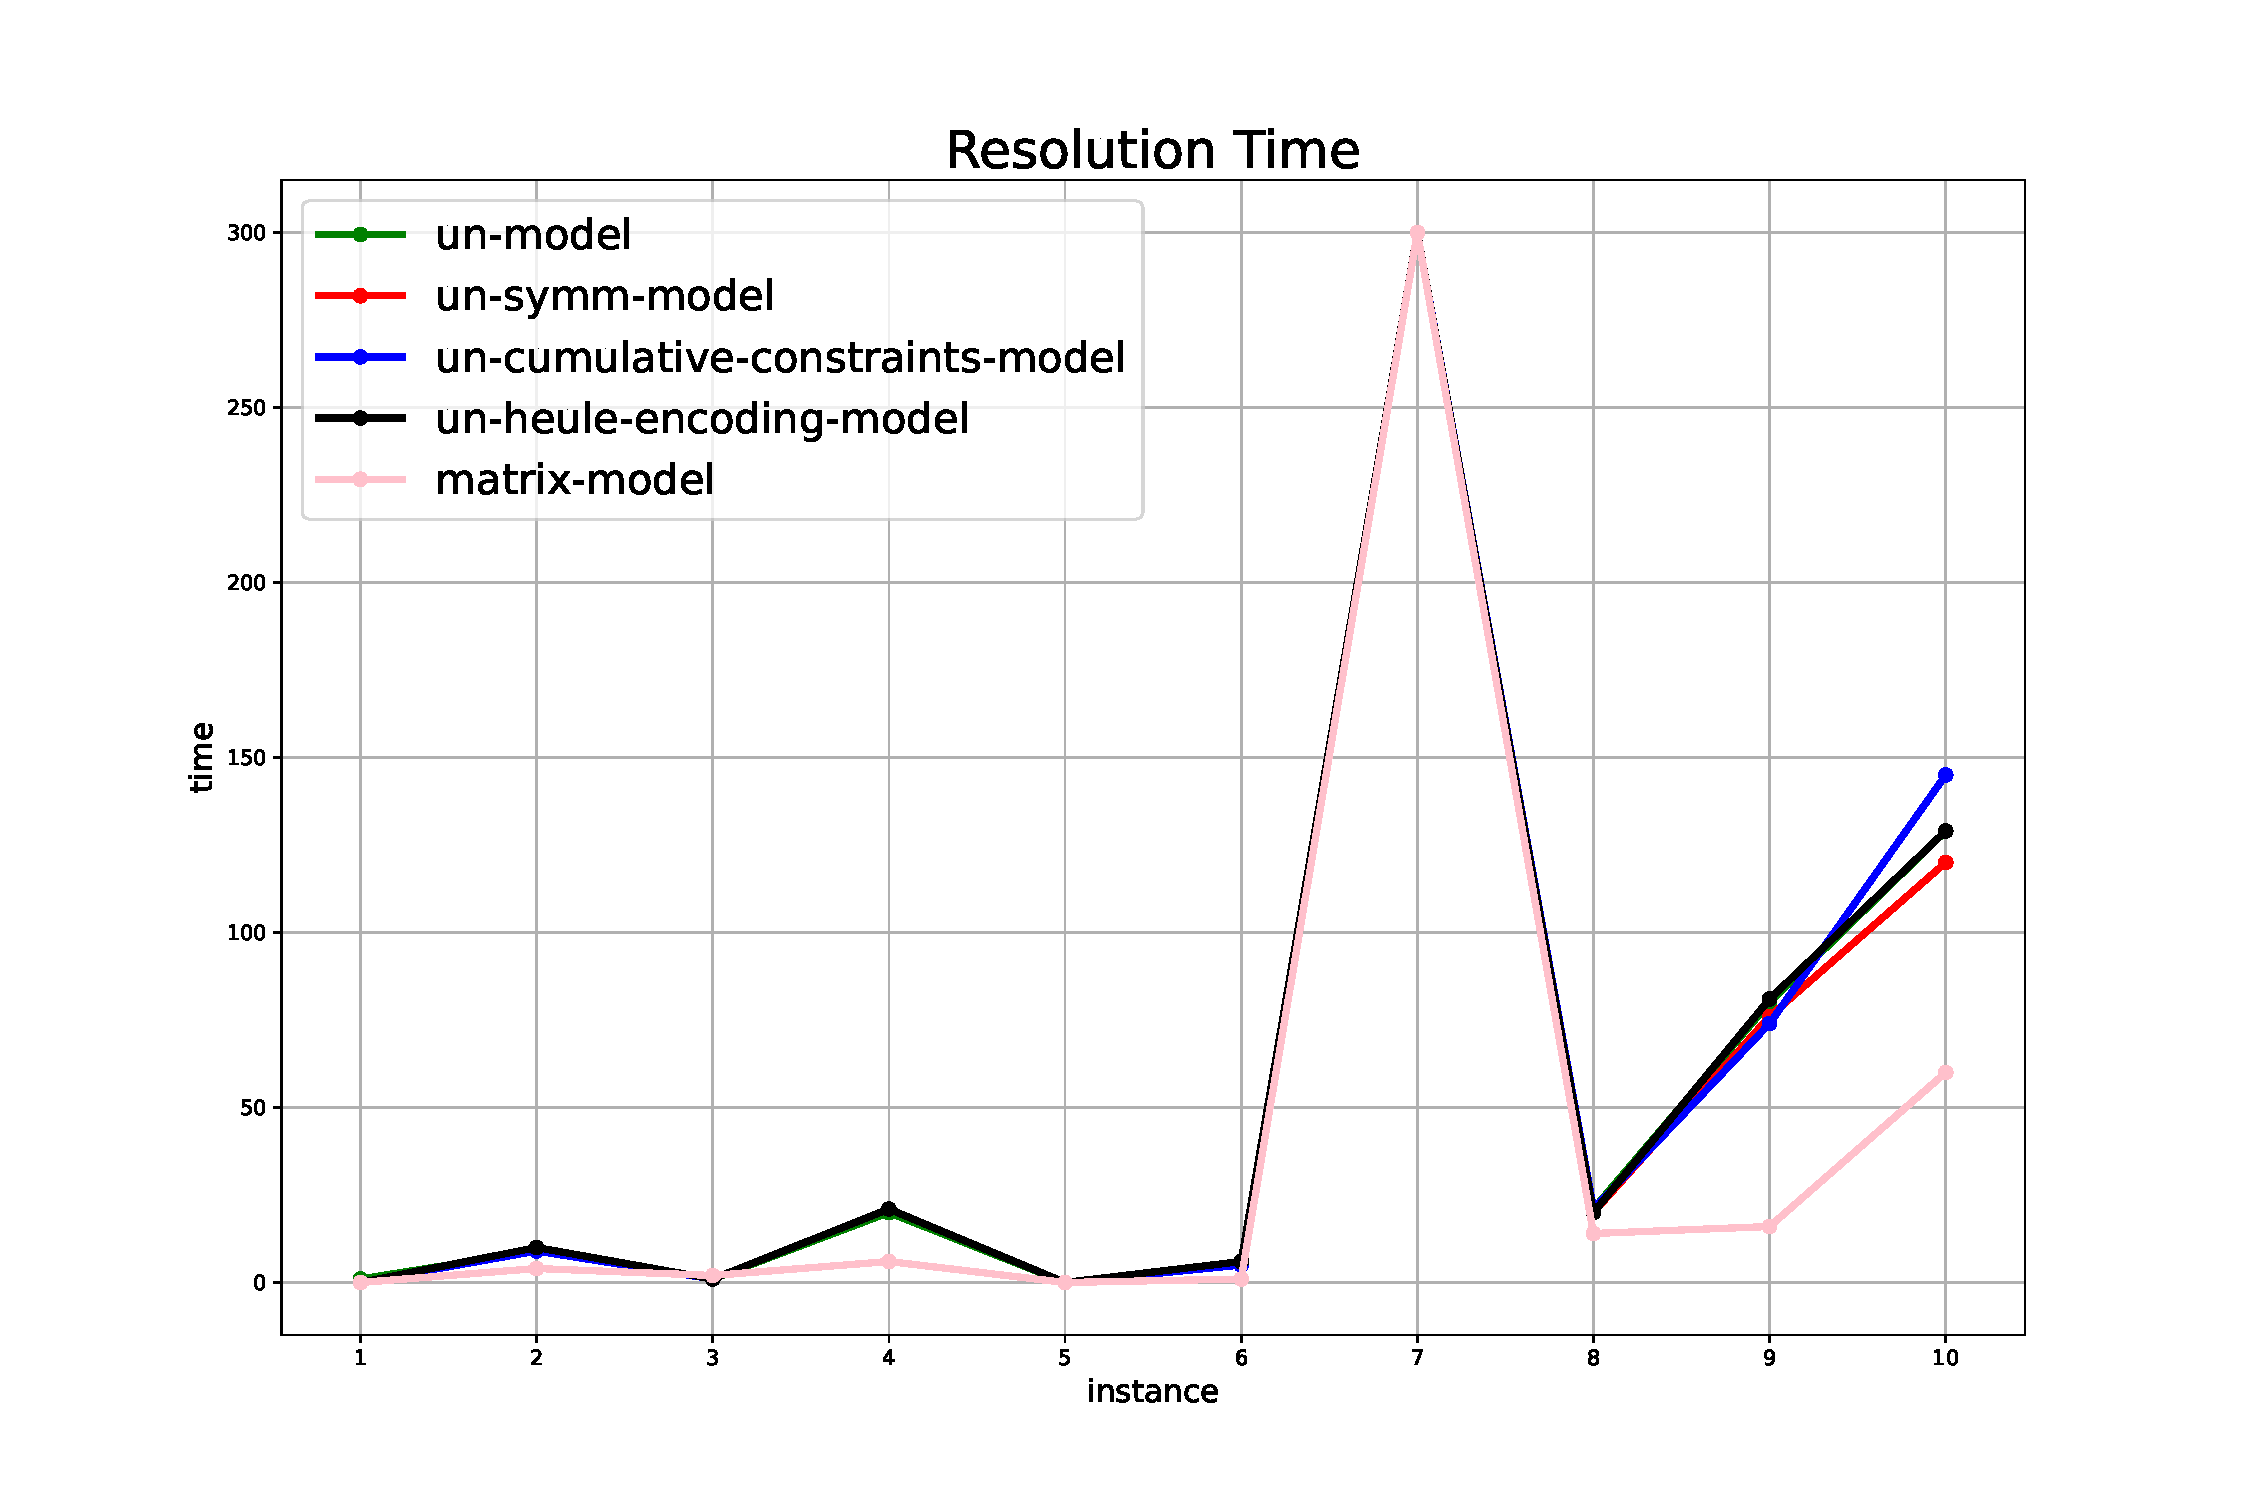
\includegraphics[width=\linewidth]{sat_images/time.pdf}
        \caption{Resolution time for each instance}
    \end{subfigure}
    \hfill
    \centering
    \begin{subfigure}{0.49\linewidth}
        \centering
        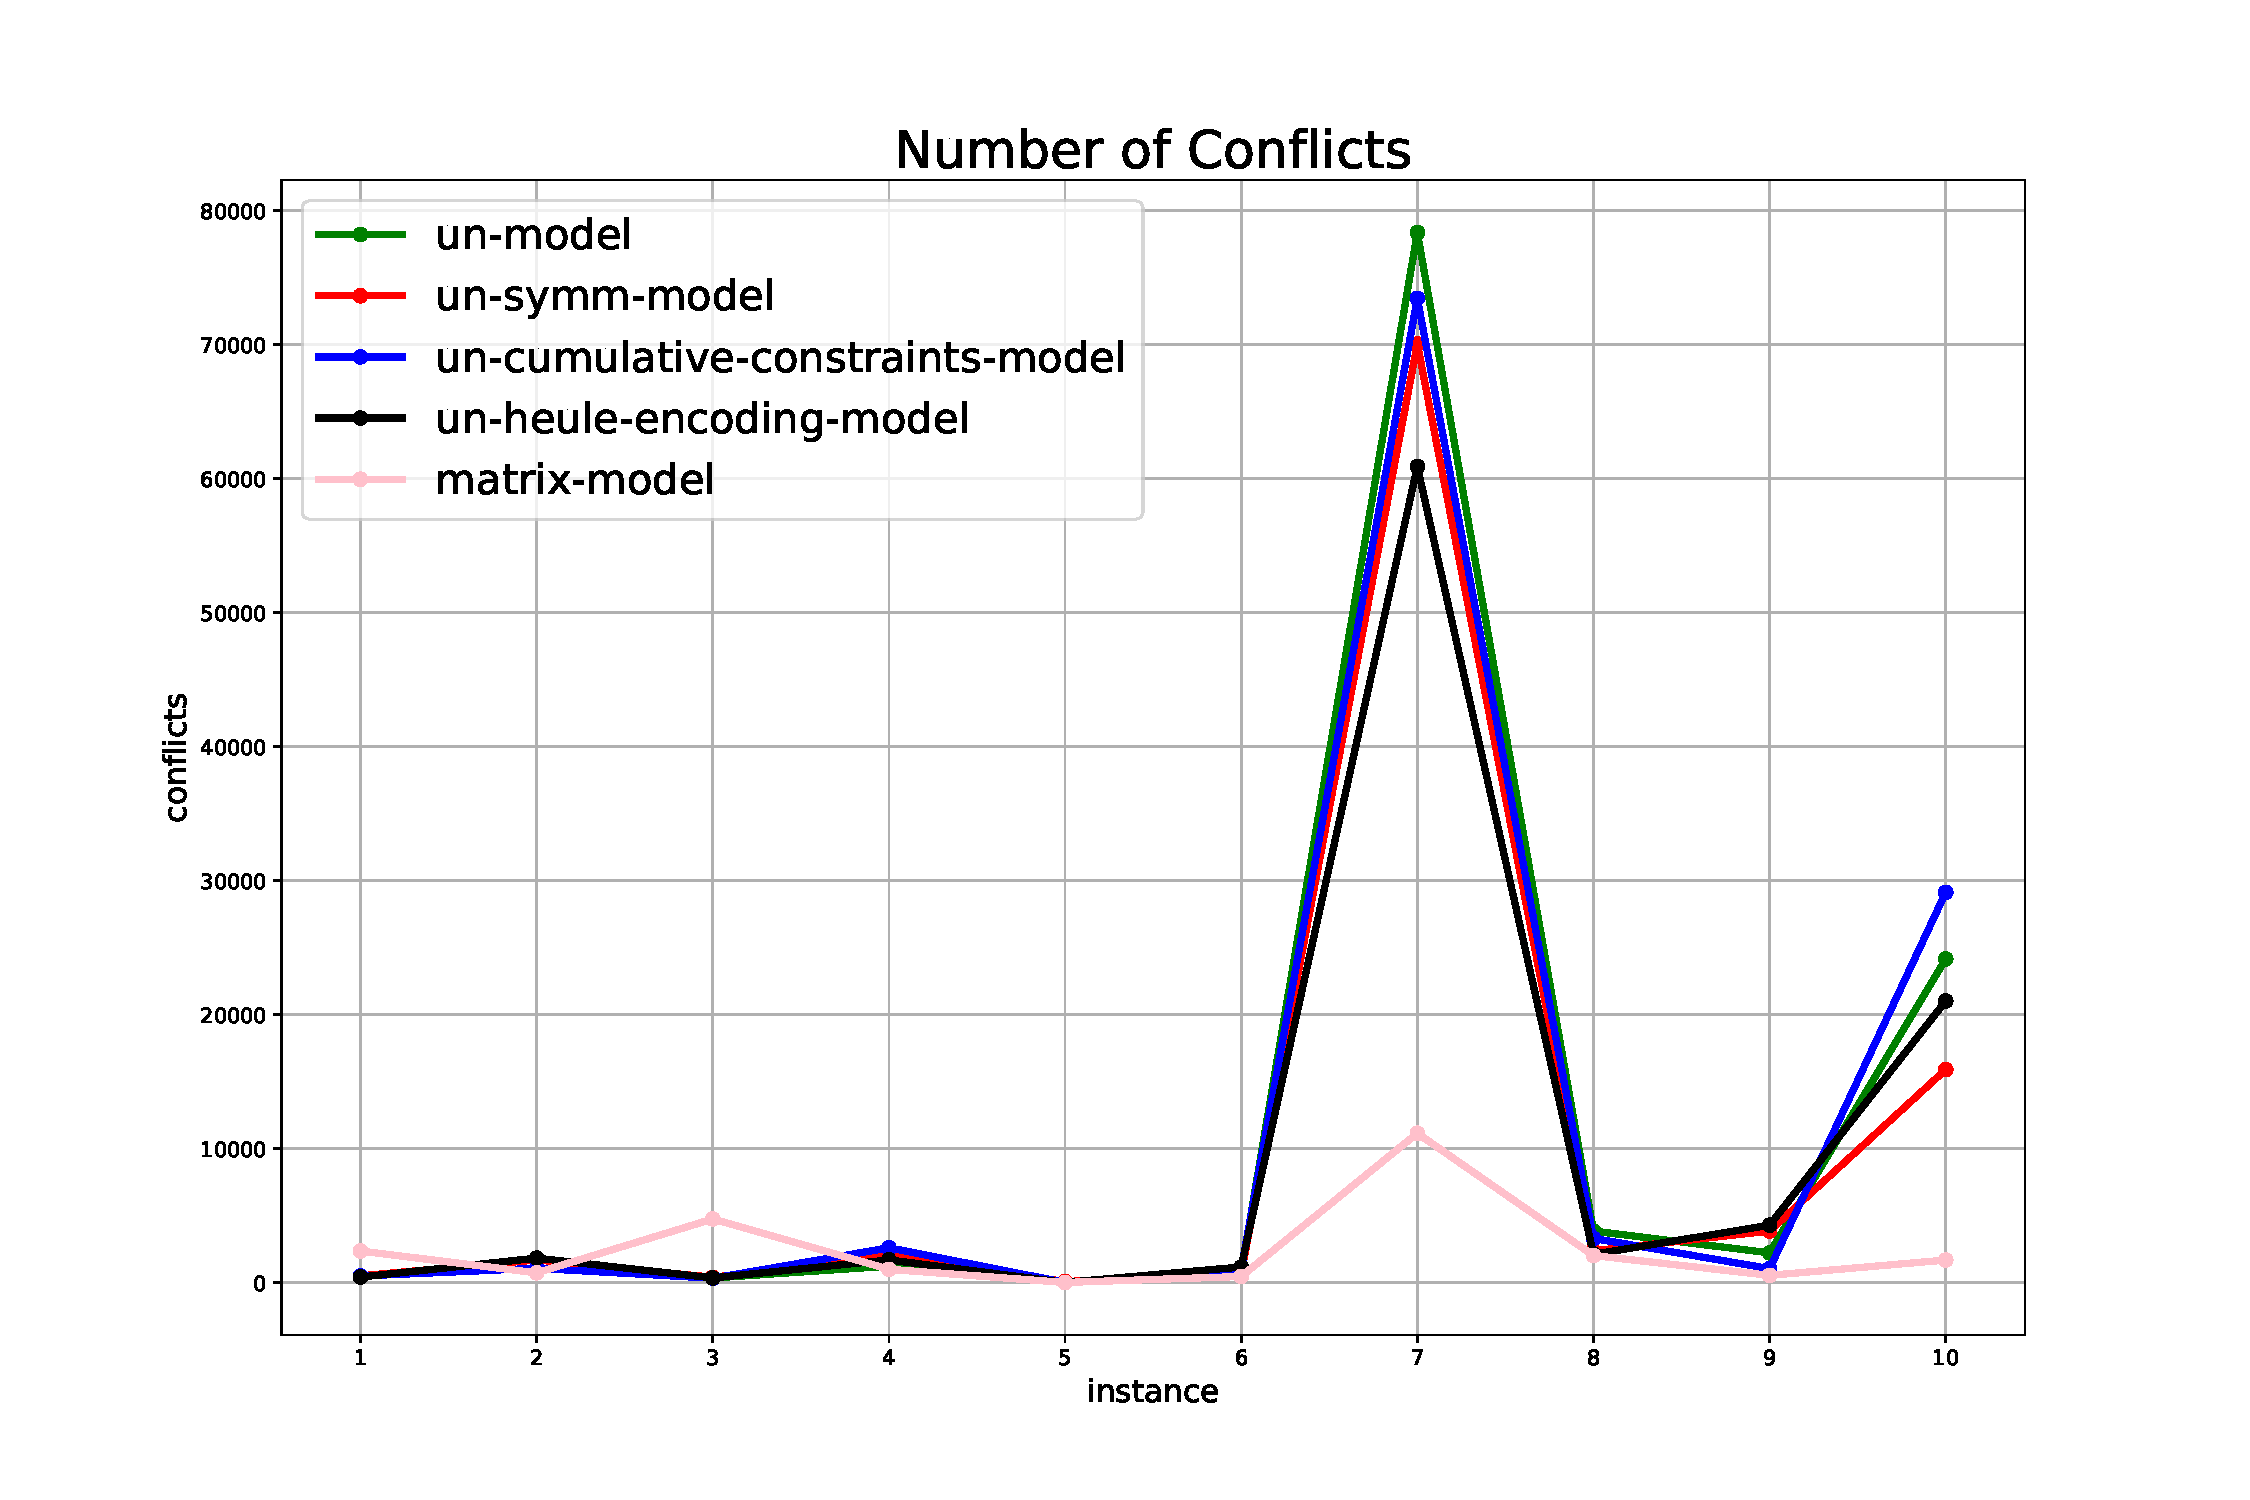
\includegraphics[width=\linewidth]{sat_images/conflicts.pdf}
        \caption{Number of conflicts for each instance}
    \end{subfigure}
    % \hfill
    % \centering
    % \begin{subfigure}{0.49\linewidth}
        % \centering
        % 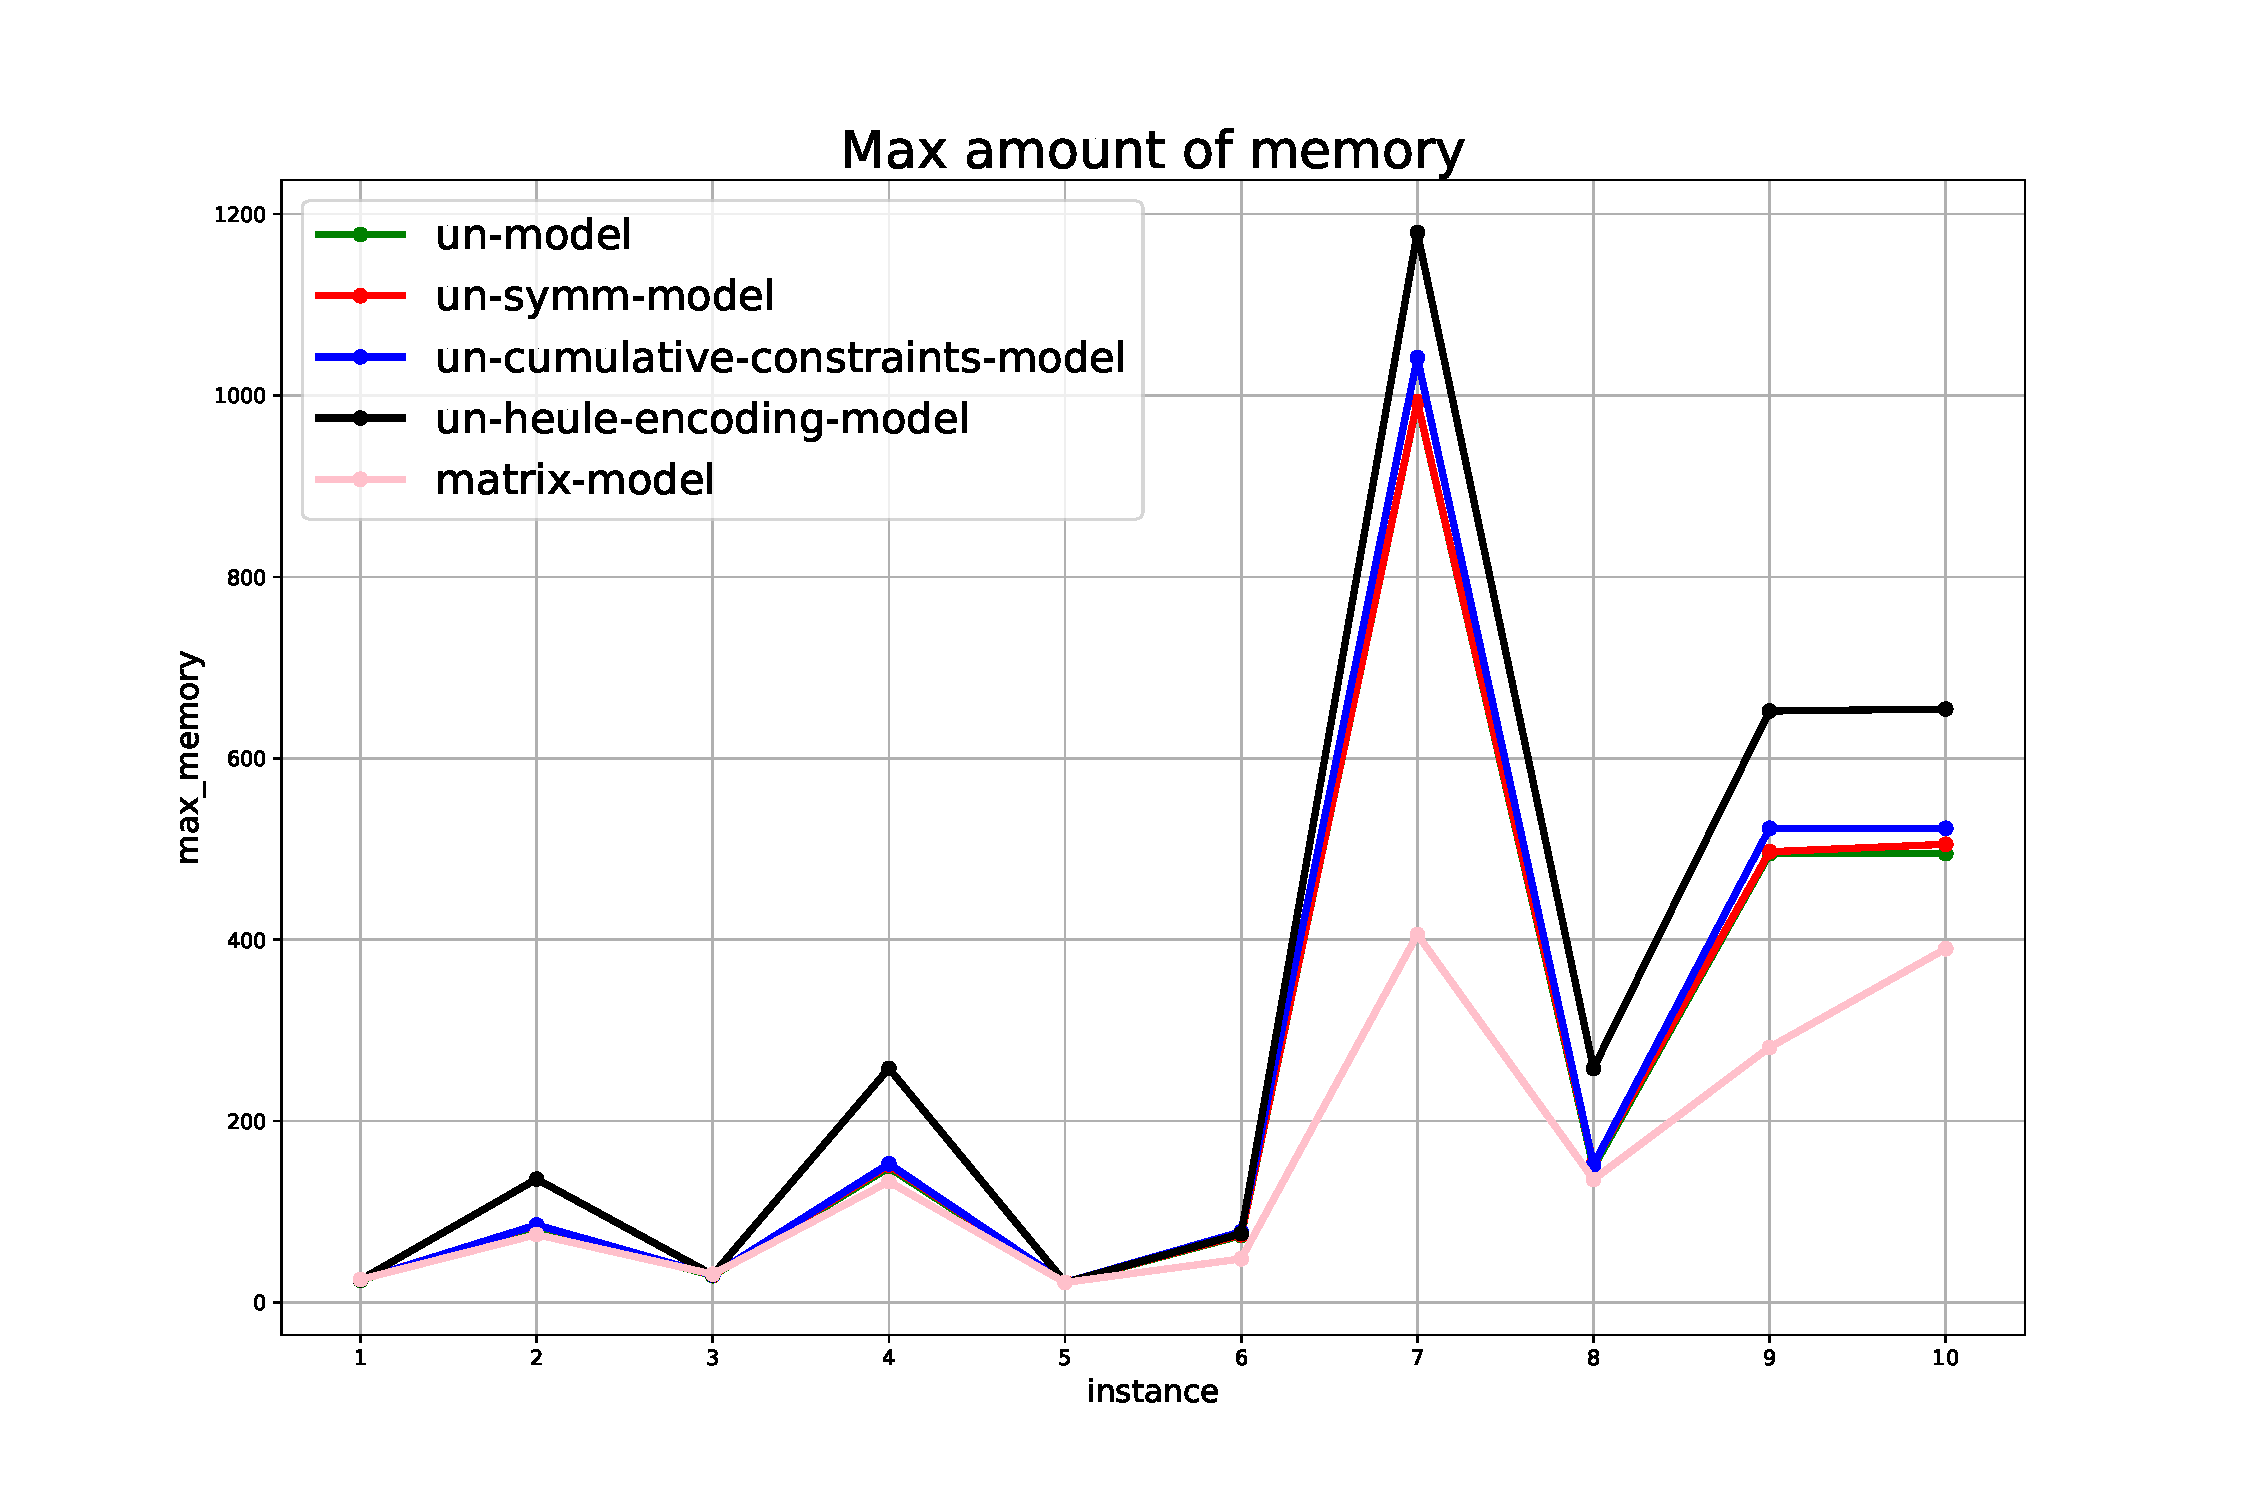
\includegraphics[width=\linewidth]{sat_images/max_memory.pdf}
        % \caption{Maximum amount of memory required for each instance}
    % \end{subfigure}
    % \hfill
    % \centering
    % \begin{subfigure}{0.49\linewidth}
        % \centering
        % 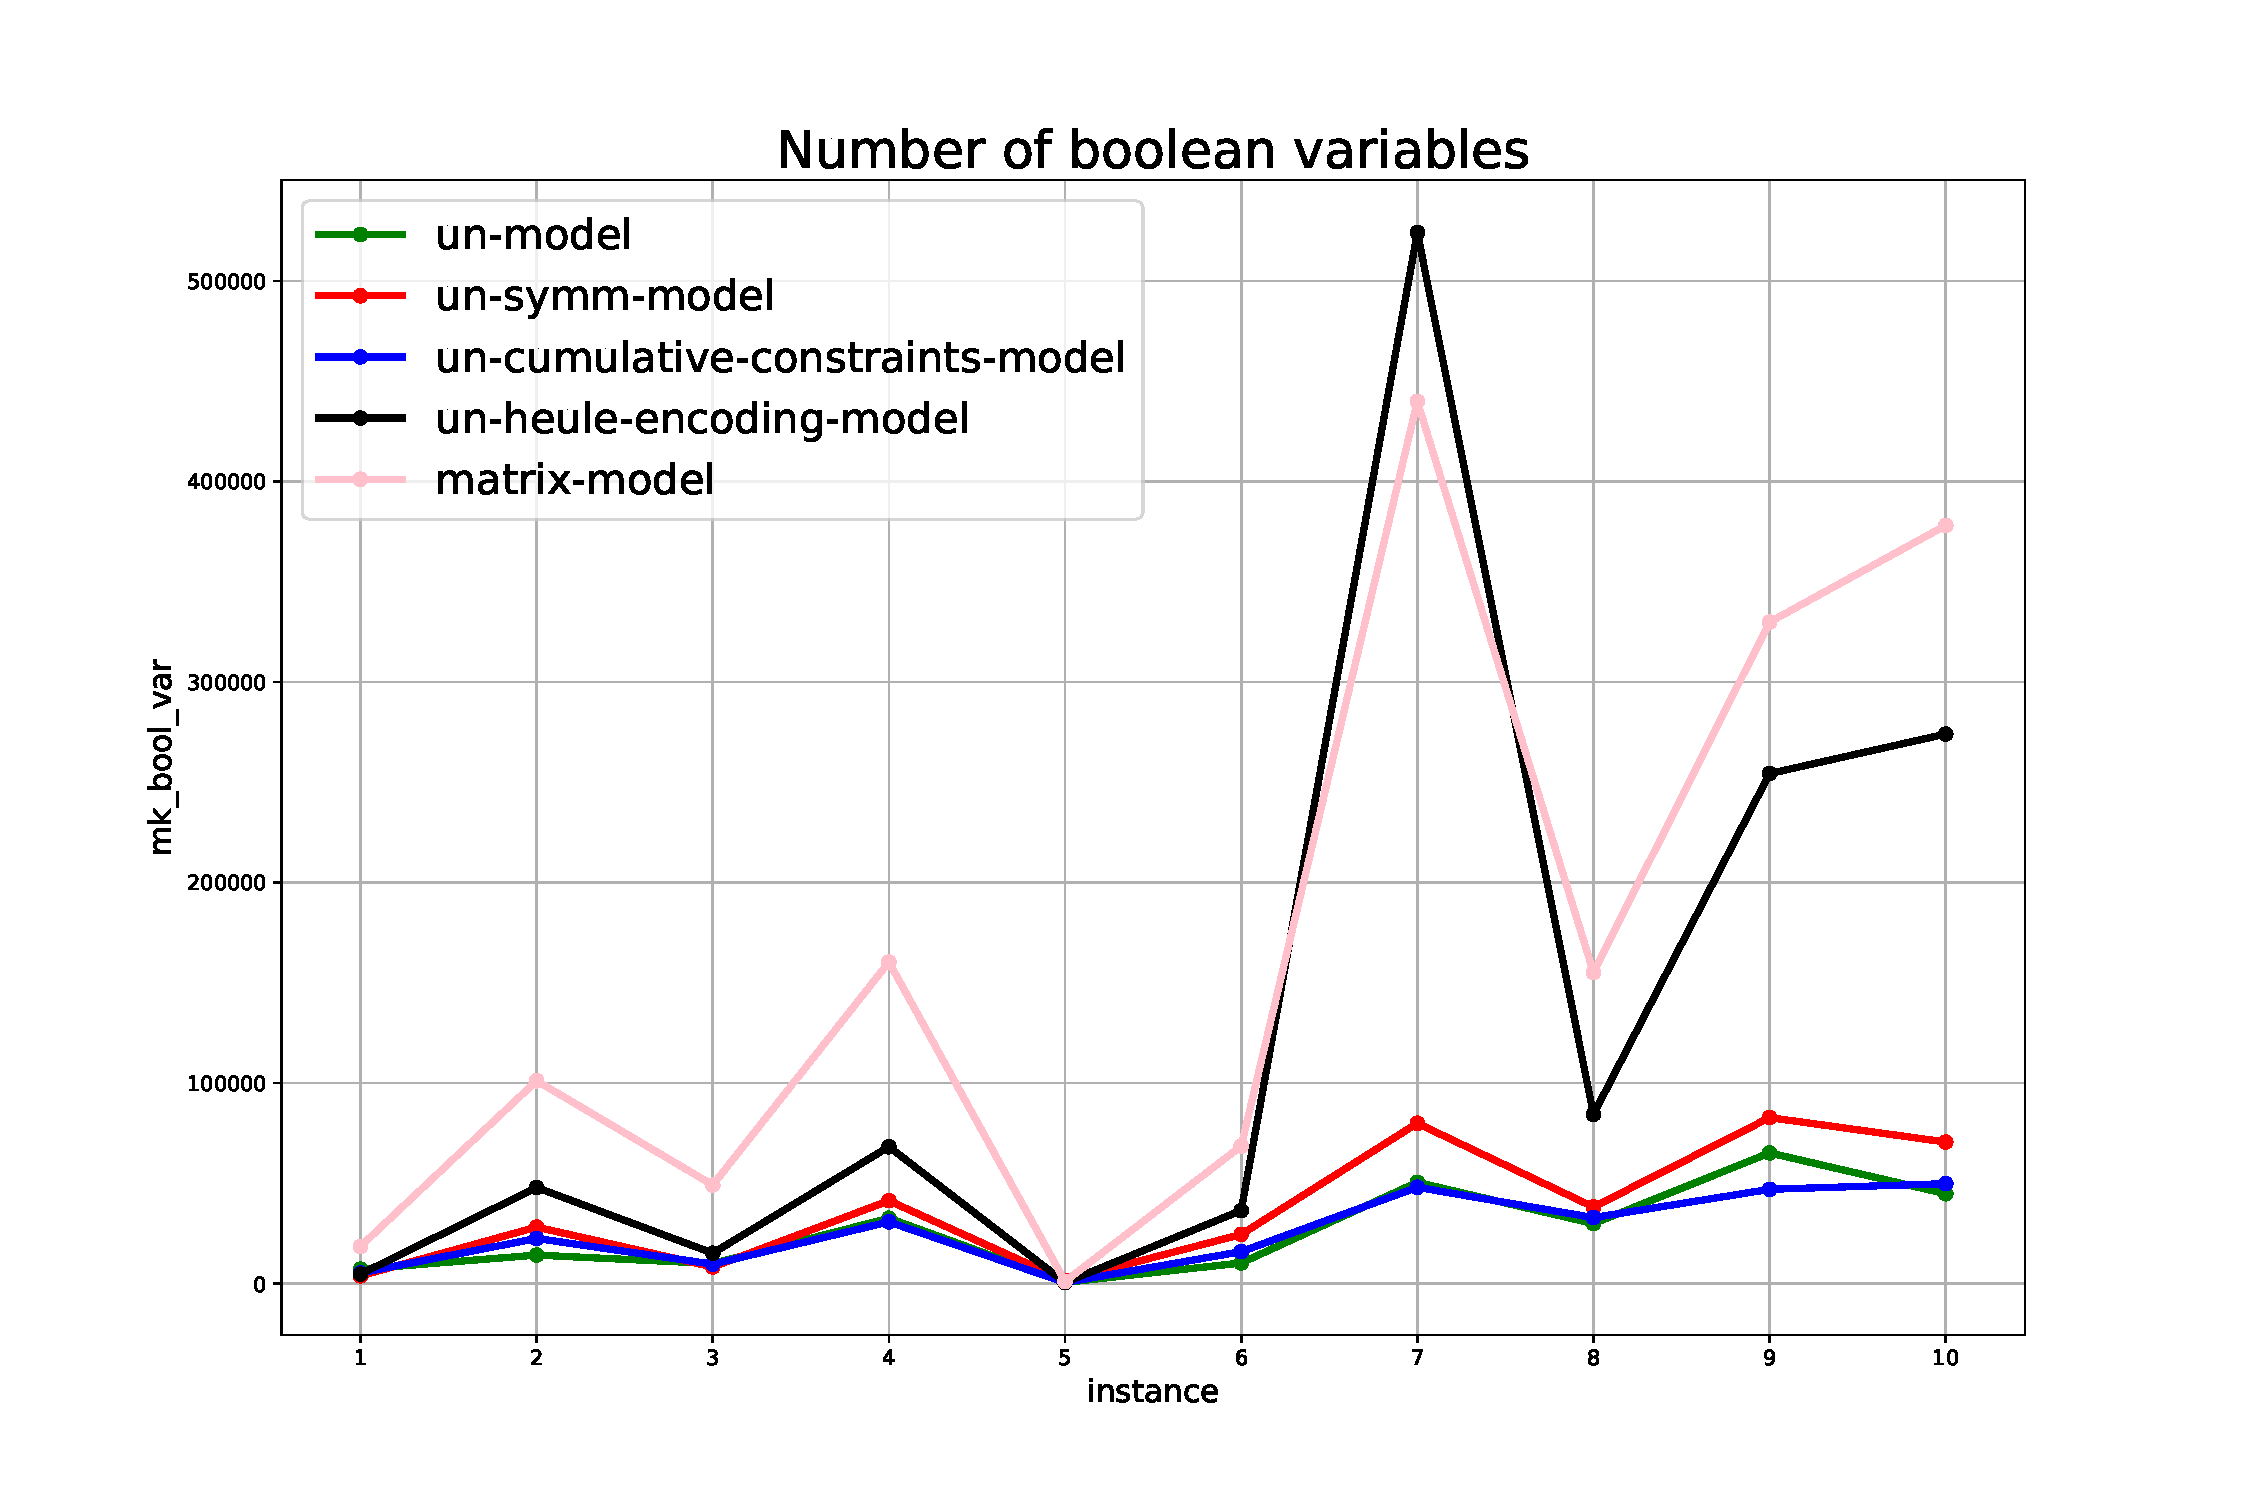
\includegraphics[width=\linewidth]{sat_images/mk_bool_var.pdf}
        % \caption{Number of boolean variables for each instance}
    % \end{subfigure}
    % \hfill
    % \centering
    % \begin{subfigure}{0.49\linewidth}
        % \centering
        % 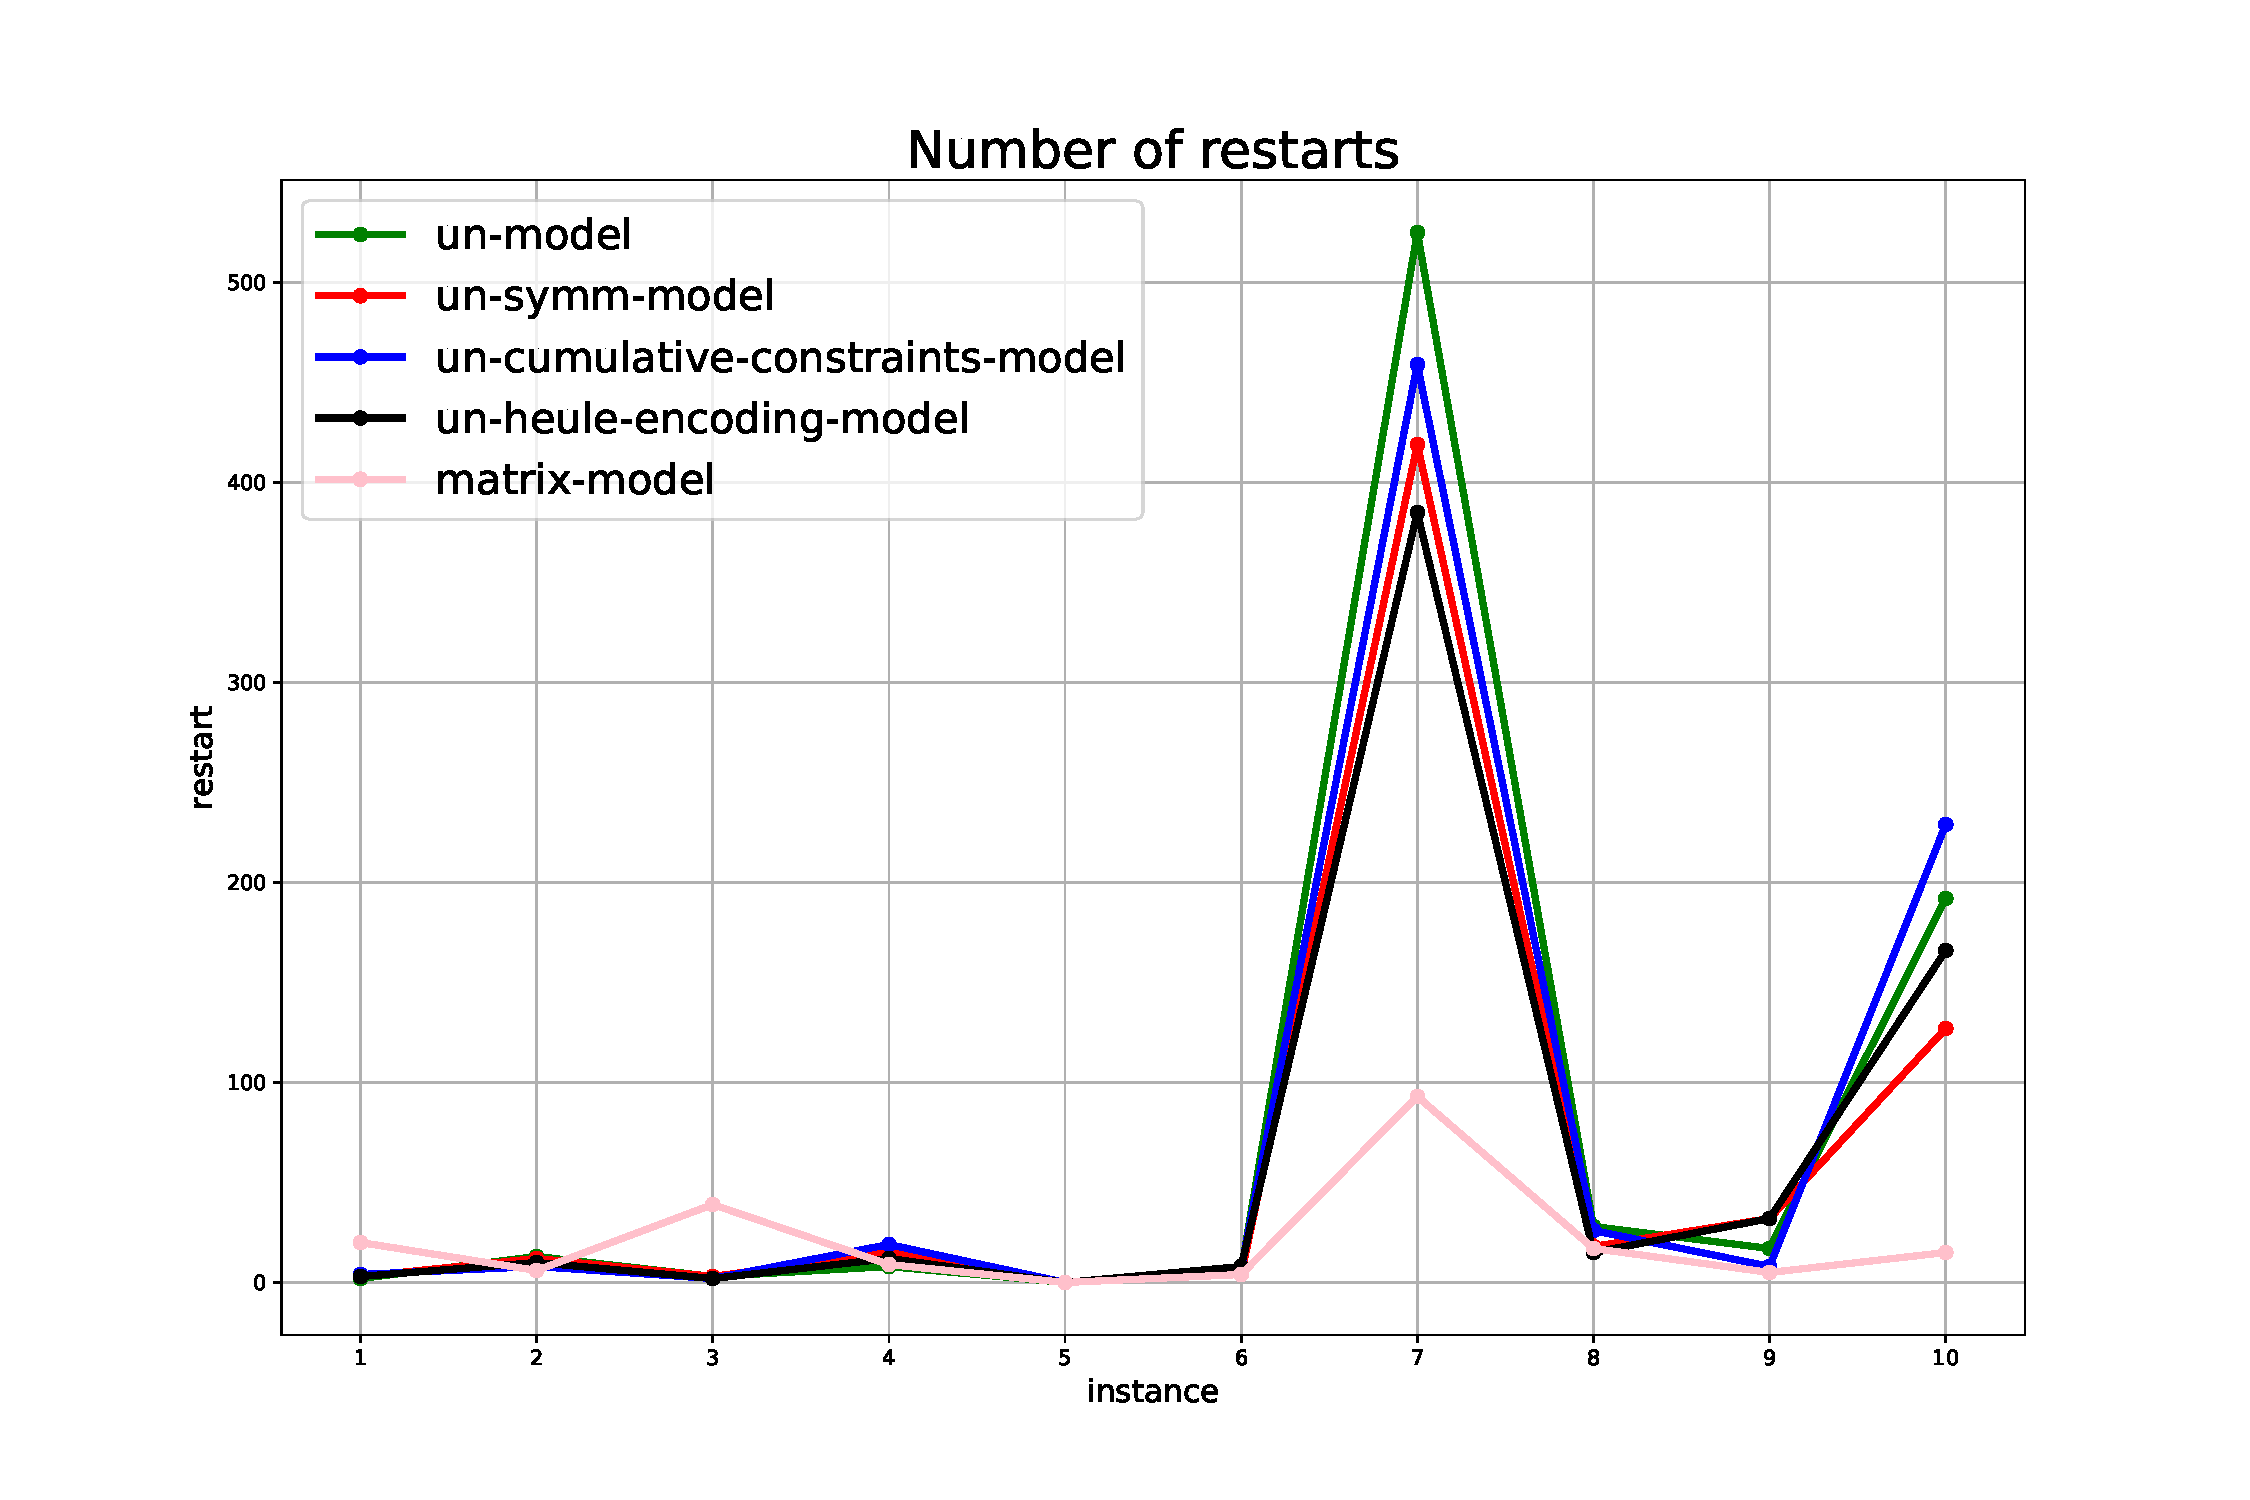
\includegraphics[width=\linewidth]{sat_images/restart.pdf}
        % \caption{Number of restarts for each instance}
    % \end{subfigure}
    \caption{Statistics about the resolution of the problem for the first 10 instances}
    \label{fig:sat_plots}\footnote{These are the only ones which reach at least a suboptimal solution.}
\end{figure}